\documentclass{article}
\usepackage[utf8]{inputenc}
\usepackage{kotex}
\usepackage{amsmath}
\usepackage{graphicx}
\usepackage{subfigure}
\usepackage{verbatim}

\title{2022 Data Structure HW11}
\author{TaeYong Kim (C011060)}
\date{\today}

\begin{document}

\maketitle

\section{Sorting Algorithms}

\subsection{Inserting Sort}
삽입 정렬은 정렬되지 않은 리스트에서 요소를 가져와 새로운 정렬된 리스트의 올바른 위치에 삽입하는 방식으로 동작하는 정렬 알고리즘이다. 이 알고리즘은 리스트의 요소를 순차적으로 검사하며, 각 요소를 앞선 요소들과 비교한다. 만약 현재 요소가 앞선 요소보다 작은 경우, 정렬된 리스트에서 올바른 위치에 삽입한다. 이 과정은 정렬되지 않은 리스트의 모든 요소가 정렬된 리스트에 삽입될 때까지 반복한다.

예를 들어, 리스트 [5, 3, 6, 1, 4, 2]를 오름차순으로 정렬하고자 하는 과정은 다음과 같다.

    1. 정렬되지 않은 리스트의 첫 번째 요소인 5를 정렬된 리스트에 삽입한다. ⇒ [5]

    2. 다음으로 정렬되지 않은 리스트의 두 번째 요소인 3을 정렬된 리스트의 첫 번째 요소인 5와비교한다. 이때 3이 5보다 작기 때문에, 정렬된 리스트에서 올바른 위치에 삽입하는데, 이는 5보다 앞서는 위치한다. ⇒ [3, 5]

    3. 이 과정을 정렬되지 않은 리스트의 나머지 요소들에 대해서도 반복한다. 

    ⇒ [3, 5, 6] (6을 삽입한 후) \\
    ⇒ [1, 3, 5, 6] (1을 삽입한 후) \\
    ⇒ [1, 3, 4, 5, 6] (4를 삽입한 후) \\
    ⇒[1, 2, 3, 4, 5, 6] (2를 삽입한 후) \\

삽입 정렬은 작은 리스트에 대해서는 간단하고 효율적인 정렬 알고리즘이지만, 리스트의 크기가 커질수록 더 이상 효율적이지 않다.

삽입 정렬의 최적 시간 복잡도는 $\mathcal{O}(n)$입니다. 이는 정렬되지 않은 리스트가 이미 정렬된 상태인 경우, 알고리즘이 각 요소를 검사하고 삽입하는데 걸리는 시간이 선형적으로 증가하기 때문이다.

삽입 정렬의 평균 시간 복잡도는 $\mathcal{O}(n^2)$이다. 이는 정렬되지 않은 리스트의 크기가 n일 때, 각 요소를 정렬된 리스트에 삽입하는데 걸리는 시간이 선형적으로 증가하기 때문이다.

삽입 정렬의 최악 시간 복잡도도 $\mathcal{O}(n^2)$이다. 이는 정렬되지 않은 리스트가 내림차순으로 정렬되어 있는 경우, 알고리즘이 각 요소를 검사하고 삽입하는데 걸리는 시간이 선형적으로 증가하기 때문이다.

\subsection{Quick Sort}
퀵 정렬은 정렬되지 않은 리스트를 정렬하는 알고리즘이다. 이 알고리즘은 다음과 같은 과정을 거친다.

1. 정렬되지 않은 리스트에서 요소 하나를 골라 기준 요소(pivot element)로 선택한다.

2. 리스트에서 기준 요소보다 작은 요소들을 기준 요소보다 작은 부분 리스트로, 기준 요소보다 큰 요소들을 기준 요소보다 큰 부분 리스트로 분할한다.

3. 기준 요소를 기준으로 왼쪽 부분 리스트와 오른쪽 부분 리스트에 대해서 각각 재귀적으로 퀵 정렬을 수행한다.

4. 왼쪽 부분 리스트와 오른쪽 부분 리스트를 합쳐서 정렬이 완료된 리스트를 만든다.

퀵 정렬은 정렬되지 않은 리스트의 크기가 커질수록 효율성이 감소한다. 그래서 퀵 정렬을 사용할 때는 기준 요소를 적절히 선택하여 최대한 균일한 부분 리스트를 만들어야 한다.

퀵 정렬의 최적 시간 복잡도는 $\mathcal{O}(nlogn)$이다. 이는 정렬되지 않은 리스트가 이미 정렬된 상태이거나 기준 요소를 적절히 선택하여 최대한 균일한 부분 리스트를 만든 경우, 알고리즘이 리스트를 정렬하는데 걸리는 시간이 log(n)의 수준으로 증가하기 때문이다.

퀵 정렬의 평균 시간 복잡도는 $\mathcal{O}(nlogn)$이다. 이는 평균적으로 기준 요소를 적절히 선택하여 최대한 균일한 부분 리스트를 만들어 정렬을 수행할 경우, 알고리즘이 리스트를 정렬하는데 걸리는 시간이 log(n)의 수준으로 증가하기 때문이다.

퀵 정렬의 최악 시간 복잡도는 $\mathcal{O}(n^2)$이다. 이는 정렬되지 않은 리스트가 내림차순으로 정렬되어 있는 경우, 알고리즘이 리스트를 정렬하는데 걸리는 시간이 n의 수준으로 증가하기 때문이다. 이는 기준 요소를 선택할 때마다 최대한 균일한 부분 리스트를 만들지 못하고, 대부분의 요소들이 하나의 부분 리스트에 속해 재귀적으로 정렬을 수행하는 경우에 발생한다.

\subsection{Natural Merge Sort}
Natural Merge Sort는 정렬되지 않은 리스트를 정렬하는 알고리즘이다. 이 알고리즘은 다음과 같은 과정을 거친다.

1. 정렬되지 않은 리스트를 읽고, 이를 여러 개의 작은 단위의 정렬된 리스트들로 나눈다. 이때 각 리스트는 자연스럽게 정렬된 상태이어야 한다.
2. 작은 단위의 정렬된 리스트들을 하나의 리스트로 합쳐 정렬된 리스트를 만든다. 이때 서로 다른 두 리스트를 비교해 각각의 요소를 선택하는 병합 정렬과 비슷한 방식으로 수행한다.

Natural Merge Sort는 입력 리스트가 이미 정렬된 상태인 경우에 효율적으로 작동한다. 이러한 점이 퀵 정렬과 달리 그렇지 않기 때문에 이미 정렬된 데이터를 자주 정렬해야 하는 경우에 유용하게 사용될 수 있다. 하지만, 정렬을 수행하는데 필요한 메모리 공간이 상대적으로 많이 필요한 단점이 있다. 또한 정렬되지 않은 리스트가 내림차순으로 정렬된 경우에는 효율성이 감소한다.

Natural Merge Sort의 최적의 시간 복잡도는 $\mathcal{O}(n)$이다. 이는 입력 리스트가 이미 정렬된 상태인 경우, 알고리즘이 입력 리스트를 읽어 정렬된 리스트를 만드는데 걸리는 시간이 n의 수준으로 증가하기 때문이다. 이는 Natural Merge Sort의 특징 중 하나로, 입력 리스트가 이미 정렬된 상태인 경우에 효율적으로 작동하는 점에서 유도될 수 있다.

Natural Merge Sort의 평균 시간 복잡도는 $\mathcal{O}(nlogn)$이다. 이는 정렬되지 않은 리스트를 입력으로 받아 정렬된 리스트를 출력하는데 걸리는 시간이 logn의 수준으로 증가하기 때문이다. 이는 Natural Merge Sort의 병합 단계에서, 입력 리스트를 여러 개의 정렬된 리스트로 나누고 이를 하나의 리스트로 합치는 병합 알고리즘이 logn의 수준으로 실행되기 때문이다. 이는 Natural Merge Sort의 특징 중 하나로, 병합 알고리즘을 사용하여 리스트를 정렬하는 점에서 유도될 수 있다.

Natural Merge Sort의 최악의 시간 복잡도는 $\mathcal{O}(nlogn)$이다. 이는 정렬되지 않은 리스트가 내림차순으로 정렬된 경우, 알고리즘이 입력 리스트를 읽어 정렬된 리스트를 만드는데 걸리는 시간이 logn의 수준으로 증가하기 때문이다. 이는 Natural Merge Sort의 특징 중 하나로, 입력 리스트의 정렬 상태에 따라 작동하는 효율성이 달라지는 점에서 유도될 수 있다.

\subsection{Heap Sort}
Heap Sort는 힙 자료 구조를 이용한 정렬 알고리즘이다. 힙은 완전 이진 트리의 일종으로, 각 노드의 값이 자식 노드보다 크거나 같은 (최대 힙) 또는 작거나 같은 (최소 힙) 조건을 만족한다. Heap Sort는 이러한 특성을 이용해 정렬을 수행한다.

Heap Sort의 절차는 다음과 같다.

1. 정렬할 리스트를 최대 힙으로 만든다.
2. 힙의 최대 원소 (루트 노드)를 추출하고, 마지막 노드와 자리를 바꾸어 힙의 크기를 감소시킨다.
3. 새로운 루트 노드를 재배치하여 힙의 조건을 만족하도록 변경한다.
4. 힙의 크기가 1이 될 때까지 2~3의 과정을 반복한다.

Heap sort의 최악과 평균 시간 복잡도는 O(n * log n)이다. 이는 정렬이 진행되는 동안 원소의 수가 n개일 때, 각 원소를 위한 비교 연산이 log n 번 수행되기 때문이다.

\section{Test Result}
다음은 본 실험에 사용된 네 가지의 데이터의 설명이다.

1) sorted : 완전 정렬된 데이터

2) partially sorted : 부분적으로 정렬된 데이터

3) random: 랜덤으로 위치되어 있는 데이터

4) decreasing: 거꾸로 정렬된 데이터

Figure \ref{table}은 각 데이터 및 각 알고리즘 별 결과 표이다. 본 실험은 학교 리눅스 서버에서 진행했다. Figure \ref{sorted}은 완전 정렬된 데이터의 각 알고리즘 별 그래프이다. Figure \ref{part_sorted}은 부분적으로 정렬된 데이터의 각 알고리즘 별 그래프이다. Figure \ref{random}은 랜덤으로 정렬된 데이터의 각 알고리즘 별 그래프이다. Figure \ref{decreasing}은 거꾸로 정렬된 데이터의 각 알고리즘 별 그래프이다. 

이러한 결과를 분석하면 다음과 같다. Inserting Sort 알고리즘은 입력 데이터 수가 증가할수록 실행 시간이 가장 오래걸린다. Quick Sort 알고리즘은 Inserting Sort 알고리즘보다 실행 시간이 증가하는 정도가 덜하지만 입력 데이터 수가 증가할수록 실행 시간이 증가하는 것을 볼 수 있다. Natural Merge Sort 알고리즘은 Quick Sort 알고리즘과 비슷하지만 실행 시간이 증가하는 정도가 조금 더 적은 것을 볼 수 있다. Heap Sort 알고리즘은 다른 세개의 알고리즘에 비해 실행 시간이 증가하는 정도가 가장 적은 것을 볼 수 있다. 따라서 Heap Sort 알고리즘은 입력 데이터 수가 증가할수록 실행 시간이 증가하는 정도가 가장 적은 알고리즘이라고 볼 수 있다.


\begin{figure}
\centering
   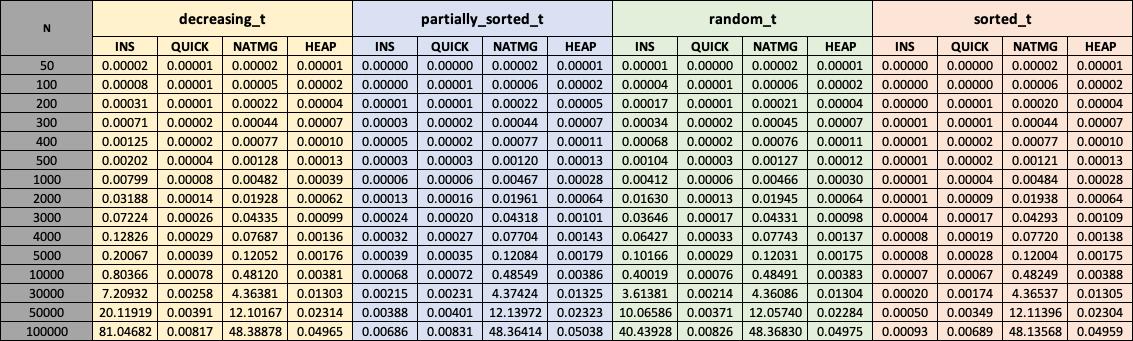
\includegraphics[width=13.5cm]{table.jpg}
   \hfil
\caption{각 데이터 및 각 알고리즘 별 결과 표}
\label{table}
\end{figure}

\begin{figure}
\centering
   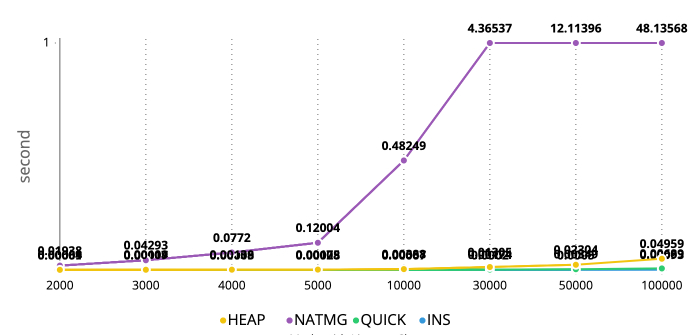
\includegraphics[width=11cm]{sorted.jpg}
   \hfil
\caption{완전 정렬된 데이터의 각 알고리즘 별 그래프}
\label{sorted}
\end{figure}


\begin{figure}
\centering
   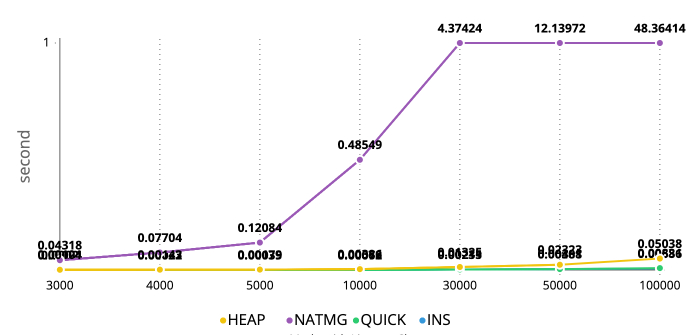
\includegraphics[width=11cm]{partially_sorted.jpg}
   \hfil
\caption{부분적으로 정렬된 데이터의 각 알고리즘 별 그래프}
\label{part_sorted}
\end{figure}


\begin{figure}
\centering
   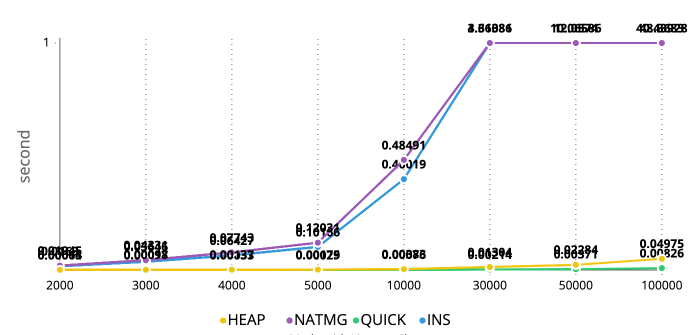
\includegraphics[width=11cm]{random.jpg}
   \hfil
\caption{랜덤으로 정렬된 데이터의 각 알고리즘 별 그래프}
\label{random}
\end{figure}

\begin{figure}
\centering
   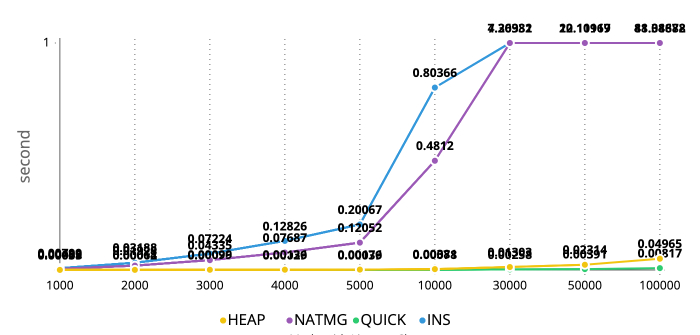
\includegraphics[width=11cm]{decreasing.jpg}
   \hfil
\caption{거꾸로 정렬된 데이터의 각 알고리즘 별 그래프}
\label{decreasing}
\end{figure}

\end{document}

